\chapter{Transformer Architecture and LLMs}\label{ch_transformers}
\chapterauthor{Jeff Yoshimi, Pierre Beckmann, Tim Meyer}{.5, .4, .1}

% LLM's browsing the net
% work in the material on random embeddings that is currently commented-out in the word embedding chapter. These are basically linear layers, that associate tokens with vectors, which can be done using one-hot inputs to select a column from a random matrix.
% Multihop reasoning
% Cite Mitchell paper: https://oecs.mit.edu/pub/00hsw4x2/release/1
% Watch new 3b1b videos and add note. (Maybe say we will do more to cohere in the next revision for better interpretation). For example, think of each head as asking a question. Gets us intuition about self attention. Also each attention head looks at something different. Queries are like questions, keys are like replies. 
% Eric S: One striking thing about GPT4 is that you can enter prompts like "Write a four paragraph essay on X" or "First, describe X. Next, describe Y. Finally, describe Z" and it will do it. By the end of the task, the prompt is rather far from the output. It would be nice if this section could explain a bit more how this architecture enables such structured outputs, which one wouldn't expect from say a next-word, next-word, next-word autocomplete on your phone. (GPT3 could also do this, unreliably, so I think the human feedback training isn't essential to this type of task, if I'm recalling correctly that GPT3 was a pure transformer without the human feedback training.)

% Discuss topics relating to BERT. (1) Encoders vs. decoders. This terminology likely comes from autoencoders, where we compress data down to a latent space and then decompress it, capturing essential information and then reconstructing it. In the context of transformers, an encoder is responsible for processing input sequences to produce meaningful representations (embeddings), which can be at the word or sentence level (refer back to the word embedding chapter). For example, we can feed a transformer encoder the first halves of hundreds of movie scripts and train it to produce the second halves, or we can train it to predict the first summary paragraph of a Wikipedia article based on the main body of the article. (2) Bidirectional vs. unidirectional is about considering the context in both directions during training. BERT considers the whole context of a token from both the left and right during training while masking specific tokens. This is known as "masked language modeling" (MLM) instead of next-word prediction.\footnote{See \cite{devlin2018bert} for a detailed explanation.} Instead of modeling language as a left-to-right stream of words, where the model predicts the next word based on the previous context (as in GPT), BERT masks a token in the middle of the sentence and predicts it based on the surrounding context. This has advantages over unidirectional left-to-right and concatenated left-to-right and right-to-left models since it creates a truly bidirectional representation where the left and right contexts are joined together. However, has faced challenges, and for some tasks, left-to-right models like GPT have been found to be more effective. I guess it's still used for some purposes but I'm not sure.

As discussed in the history section \extref{age_generative_ai}, we have entered a new stage in the history of neural networks, what we are calling the ``age of generative AI'', which should be familiar to you via such tools as ChatGPT. In their most familiar form, these transformer-based large language models (LLMs) generate text responses to text inputs by repeatedly predicting the next word or token in a sequence.\footnote{The concept of token is introduced in chapter \extref{ch_word_embeddings}. Following practice introduced there we will vacillate between ``token'', which is more accurate (since it encompasses punctuation, word parts, and other non-word entities) and ``word'', which is more intuitive.} They are trained on large datasets of everyday text, like text from the internet, which is easily available. As noted in section \extref{age_generative_ai}, it is common to equate ``transformer'' with ``LLM'', but the two concepts are distinct. The transformer is the neural network architecture, while an LLM is just any model of language generation that is based on a large dataset. An LLM can be built out of something besides a transformer, and transformers can be used on things besides language. For example, some state of the art image classification models are now transformer-based, and OpenAI has released an impressive video generation model – Sora, which also runs on a transformer architecture. However in this chapter we focus on transformer-based models of text generation like GPT.\footnote{There are many other models in this class. As of this writing (June 2024), this includes the open Ai GPT series: GPT, GPT2, GPT3, GPT4, and GPT 4o. It also includes BERT (Google’s first LLM, which is now out-dated), Gemini (Bard), several Claude models (Anthropic;  semi open-source), Llama, LLama2 and LLama3 (Meta), and Alpaca (Stanford; open source). Most of these models can only be accessed online but some can be downloaded and run locally, further fine-tuned, etc. A list of LLMs ranked by how well they chat is here: \url{https://chat.lmsys.org/?leaderboard}.} We will sometimes refer simply to ``LLMs'' by which we mean transformer-based LLMs.\footnote{There are numerous high quality online resources for learning about LLMs. An excellent visual introduction is at this website: \url{https://poloclub.github.io/transformer-explainer/}. Three blue one brown is always excellent on visual intuition and he has a \href{https://www.youtube.com/watch?v=wjZofJX0v4M&list=PLZHQObOWTQDNU6R1_67000Dx_ZCJB-3pi}{\underline{youtube video}}. For a more technical walk through on building an LLM from scratch see \href{https://www.youtube.com/watch?v=kCc8FmEb1nY}{\underline{Karpathy's tutorial}}.}
%  GPT as a generic term means “Generative Pre-trained Transformer” (though it is often also used to refer specifically to open AI’s models. Though the transformer architecture can be used in many ways, it became prominent through its use to support large language models (LLMs), which are language models that generate human readable text.}

Earlier efforts at text generation and natural language processing used supervised recurrent networks (chapter \extref{ch_supervised_recurrent}), which are, as we saw, in various ways limited. In particular, they can only process a small amount of context, and suffer the vanishing gradient problem. The transformer architecture is basically a very complex feed-forward network that facilitates contextual representation that can be aware of multiple kinds of relationships between arbitrarily far-flung parts of an input stream. Because it is a feed-forward network, many of the older techniques covered in this book can be applied to the architecture. In particular, all the lessons of the deep learning revolution (section \extref{deep_revolution}) apply here, and indeed, transformers are many-layered deep networks (chapter \extref{ch_cnn}) that make good use of both \glossary{representational width} and \glossary{representational depth}. They can be trained on large datasets using highly optimized parallel hardware. Like all the other networks discussed in this book, they are not just useful as engineered tools, but are highly relevant both to neuroscience and cognitive science, and seem to develop meaningful internal representations. 

We start with preliminary discussion of how transformer-based LLMs are trained using highly available text data, and how a special recursive trick can be used to make a feed-forward network that only predicts next words still produce meaningful conversational outputs. We then discuss how the transformer architecture itself works. Finally we consider how LLMs are utilized and evaluated and the relevance of these models to cognitive science, neuroscience and other areas.

Changes in this area are rapid, and the relevance of these areas to cognitive science is only now being studied, so updates to this chapter are expected.

\section{Learning to speak Internetese}

In section \extref{languageModelsRecurrent} we saw how recurrent neural networks trained on example text can learn to speak in a way that reflects the statistical properties of the training data. A network trained on Shakespeare will start to speak fake Shakespeare, a network trained on real math can generate fake math, etc. Large language models using transformers do the same thing, they just do it much better. The architecture is better suited to the task, as we will see, and they can use much larger datasets (hence ``large'' being added in front of ``language model''). In fact, the training set for GPT-3 (an early LLM) was not all of Shakespeare, or just a bunch of math papers, but rather a large subset of the \emph{entire internet}, which included all of Wikipedia, a few compilations of books, and a web-scraped archive of the internet called ``common crawl'' (\url{https://en.wikipedia.org/wiki/Common_Crawl}). See figure \ref{gptDatasets}. Similar datasets continue to be used on LLMs, so if you've ever written anything online, there is a decent chance it is part of the training data for one of these models. 

Since all of Shakespeare is on the internet, and discussions of every topic of human endeavor from physics to history, and plenty of gossip and randomness about popular culture and everything else, these models can talk about all of these things. They can statistically generalize from their training data, which consists of a large part of the internet, which in turn encompasses many of the books and recorded knowledge of human history. In a sense, these models learn to speak ``internetese''. 

\begin{figure}[h]
\centering
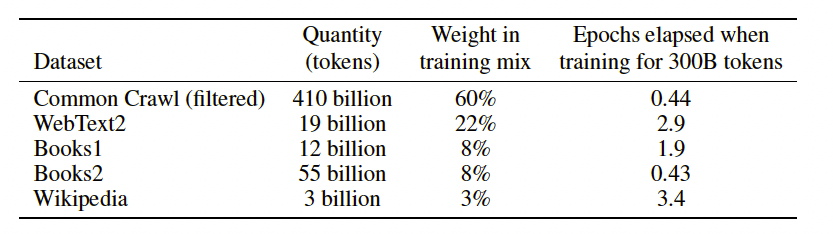
\includegraphics[scale=.4]{./images/gptDatasets}
\caption[From \cite{brown2020language}.]{The datasets used to train GPT-3. The data mostly consists of data scraped from the internet, but lots of books and all of Wikipedia are also included.}
\label{gptDatasets}
\end{figure}

The results are impressive. The texts these models produce are no longer obviously fake in the way the examples from section \extref{languageModelsRecurrent} were. In fact, in some cases they arguably pass the \glossary{Turing Test}, a long-standing test for artificial general intelligence, answering questions and producing convincing  text in response to prompts. Whether LLMs really pass the test is a matter of ongoing controversy. This is discussed further in section \ref{llmPhilosophy}.

\section{Training Using Next-Word Prediction}

Recall from chapter \extref{ch_data_science} that a training dataset consists of inputs and targets, and is also called a labeled dataset. As noted there, this kind of labeled data can be hard to obtain. We might have lots of pictures of people but not know the names or identities of the people in the pictures, or lots of pictures of cats and dogs but not whether a given picture is a cat or dog. Creating targets for a large dataset is labor-intensive, requiring humans to manually label each picture.

% Need a bit more fanfare on the embedding step, since it is the first step in the pipeline, but not sure the best way to integrate it into the discussion
LLMs like GPT use a special method (sometimes known as auto-regression) to take \emph{any piece of text} and convert it into a training data set. The trick is, roughly, to treat a given string of text tokens without the last token as an input, and then to treat the final token as a target or label. More specifically we use vector embeddings of the tokens. The amazing thing about this method is that it can be used to take \emph{any text} as a training dataset. No longer do we have this difficulty of finding labeled data. Just take any old piece of written text, and you've already got multiple training examples, just by taking concatenated vector embeddings different sequences of tokens as input and vector embeddings of the next tokens after those sequences as targets.

For example, consider this block of text adapted from the Wikipedia page for UC Merced:

\begin{quote}
The University of California, Merced is a public land-grant research university in Merced, California. It is one of the ten campuses in the University of California (UC) system. Established in 2005, Merced is the newest campus within the UC system.
\end{quote}

From this, we can create a bunch of training examples, a list of input / target pairs. We might use ``The University of" as an input, and then ``California'' as a target. We simply associate each token in the input with a vector using a word embedding (chapter \extref{ch_word_embeddings}). (The target is also vector encoded, but in a different way; we discuss this in section \ref{llmOutput}). Using the word we can build a table of input-target vector pairs, which we can use to train a feed-forward neural network. For a sense of the idea, see figure \ref{nextWordPrediction}.\footnote{Note that normally a word like ``University'' would be split into multiple tokens, but we are keeping things simple here. Some information tokenizers is in chapter \extref{ch_word_embeddings}.} 

\begin{figure}[h]
\centering
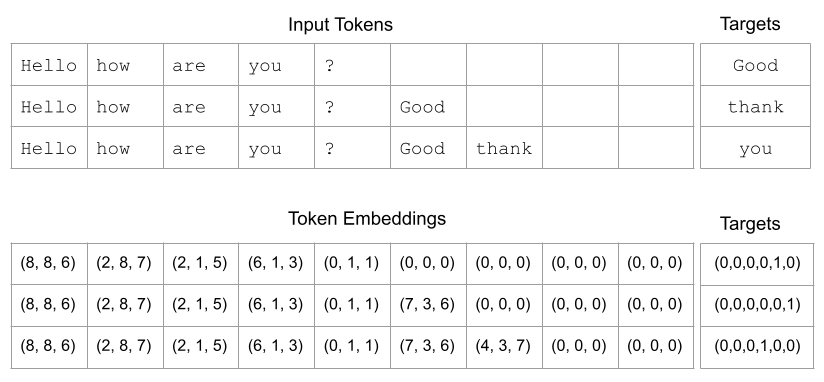
\includegraphics[scale=.45]{./images/contextWindow.png}
\caption[Jeff Yoshimi]{How text sequences can be converted into training datasets for large language models. A set of tokens is converted into vectors using a token embedding (the vectors shown are arbitrary, just to illustrate the idea). We can treat each concatenated partial sequence of token embeddings as an input and the next token as a target for the supervised learning algorithm. }
\label{nextWordPrediction}
\end{figure}

Note that the word embedding in this example is 4-dimensional (each token is associated with an array of 4 numbers, a vector in a 4d space). In real LLMs this ``embedding dimension'' is quite large, for example over 12,000 for GPT-3 (see figure \ref{gptParams}). 

In practice, a sequence of tokens is converted into a matrix where each row corresponds to the token embedding for one token. This idea is illustrated in section \extref{wordEmbeddingMatrix}, where it was described as a ``token embedding matrix''. This stack of vectors is ready to be processed by the LLM.\footnote{What is actually fed to the transformer is  a batch of these token embedding matrixes, that is a rank-3 tensor (see section \extref{sect_tensors}).}

One interesting feature transformers is that the processing they do does not inherently care or know about the order of tokens in a sequence. Thus, the tokens in a token embedding matrix are in a sense unordered (their position in a stack is an order, but this information is not easily available to the network given how it processes information), which allows for super-fast parallel processing. Thus a \glossary{positional encoding} is used to modify the vectors in a token embedding matrix, often by using a trigonometric function that simply adds more or less to the numbers in the vectors depending on where they are in a sequence.\footnote{This is a kind of feature engineering trick; see chapter \extref{ch_data_science}.}  In figure \ref{transformerBlockSimple} the encoding subtracts 1 from each component of the word embedding for ``Hello'' (which was $(8,8,6,1)$ for the sample embedding in figure \ref{nextWordPrediction}).
  
\section{How Text is Generated from a Feed-Forward Network}

% Pictures needed for recursion trick and context window. E.g take second figure in this chapter and add some arrows or numbers showing how to generate sequences.

One confusing thing about figure \ref{nextWordPrediction} is that we go from a large input covering a whole set of tokens to a single token as output. So great, we can predict single words. But how do we go from single words to generating long text outputs, or having conversations? In fact, in hearing about generative AI as ``next word prediction'' machines, you may have sometimes wondered how such complicated things can happen when all they model does is predict next words.

The answer is by using what we can call the ``recursion trick''. This trick allows us to take a feed-forward network that only predicts next words and use it to produce streams of text output. In fact, it's remarkably simple. We feed a network a set of inputs corresponding to string of text, and it produces an output corresponding to the predicted next token. That output is then appended to the previous input, and this longer input is now fed back to the network. This process is repeated to produce a stream of text outputs. This technique can be used to generate unending sequences of text from any prompt.\footnote{Notice that this is a kind of recurrence, and arguably this makes LLMs used in this way a kind of recurrent network. Outputs are fed back in as part of inputs. However, the outputs are text which then must be converted back to text inputs which are then vector encoded. In fact, recurrent networks were originally used for text processing, as we saw in chapter \extref{ch_supervised_recurrent},but it turns out fancy feedforward networks used in this way outerperform them. (In those cases a vector representation of each token in the sequence would be presented separately: ``hello'', ``how'', ``are'', ``you'', and ``?''.).} The prompt is our input, and then answers are generated using the recursion trick. Text will continue to be generated until a special end of sequence token is reached.\footnote{It was an important step forward with GPT-3 when the ability to produce end of sequence tokens in a way that mimic human conversation or ``chat'' was produced. This was done using special training techniques, in particular, RLHF, reinforcement learning with human feedback. RLHF uses reinforcement learning and policy gradient descent, with a human in the loop. This was introduced with GPT-3.} 
% Eric S: Could probably use a section on the role of human feedback in the final stage of model development. So promote this note.

So this gets us one response. But then you type a new question. That \emph{entire question} is appended to the \emph{entire past conversation} including both what you and GPT have said so far. 

Suppose, for example, we want to ask a network ``hello how are you?'' The input to the network is the whole sentence $\{$``hello'', ``how'', ``are'', ``you'', ``?''$\}$. Let's  not worry about the vector embeddings, and just see the general idea, as shown in figure \ref{gptRecursedInputs}. Notice that the initial prompt is the initial input, but then the prompt \emph{and} the first word of the response are used as the next input, and this process can be repeated until a response is written out.
  
\begin{figure}[h]
\centering
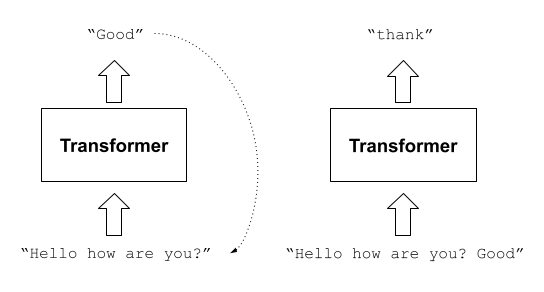
\includegraphics[scale=.7]{./images/gptRecursedInputs.png}
\caption[Jeff Yoshimi]{A schematic view of how ``conversations'' are generated from a feed-forward network in systems like GPT. The output from one moment is added to the end of the input, and the new input is then fed in. The process is repeated to generate a full response.}
\label{gptRecursedInputs}
\end{figure}

Of course, as we keep doing this, the inputs to the network get larger and larger, and there must be some limit to how far we can go, right? The answer is yes. Any LLM specifies a fixed length \glossary{context window}. At the start of a session, this window is mostly zeros, except for the initial prompt. In a dialog, the prompts from a person and the responses from the LLM are both included until the context window is filled. Thus, if the context window is large enough, whole series of back and forth conversations can be processed. All the prompts and responses up until the current point are part of the input, and then the LLM uses the recursion trick to generate new responses that are sensitive to everything that's been discussed thus far. When the system runs out of slots in its context window, items are simply removed from the start of the context window (from a computer science standpoint, this is a queue). This is intuitive in figures \ref{nextWordPrediction} and \ref{gptRecursedInputs}. These context windows can be remarkably large. GPT-3 has a context window of about 2000 tokens or about 6 pages of text, and early versions of GPT-4 had context windows of 32,000 tokens or about 72 pages of text. 

\section{The Transformer Architecture}\label{transformers}

We have thus far covered high-level features of how LLMs work, but have treated the transformer as a black box. The time has come to open the box. How does the fancy feed-forward network at the heart of these models work? Its power rests on a few novel architectural innovations, which combine representational width and representational depth with a special form of context awareness. All the things we've seen about other neural networks apply here. It is a kind of deep feed-forward network, which uses a huge amount of training data. But the key innovation is that within each ``layer'' it can develop many forms of context representation, which relate all the tokens in a context window to each other.

\subsection{Blocks}

% This big pass is coming esp. here. One thing to possibly do is to show the embedded tokens stacked in matrix form so it's clear the embedding is done with matrix operations. This also needs to  be cohered with the NLP chapter.

% Eric S below: "Compares" is vague. How to give a sense of it right up front
The transformer architecture \cite{vaswani2017attention} contains layers or ``blocks'' which are specialized to process the large context windows that are fed to the network as input. With training they learn to find long-range dependencies between different parts of a context window. Recall that the context window  includes an original prompt, its own response to that prompt, etc.; it includes the \emph{entire exchange} you've had with GPT up to the current point, so long as it fits in the context window. Each block combines a ``self-attention'' layer with a traditional linear layer and several other mechanisms (see figure \ref{transformerBlockSimple}). The self-attention layer is where the magic happens. One part of this layer compares each token in the context window to every other token in the window. In our simple example, ``hello'' is compared to ``how'', ``are'',  ``you'', and also to itself. These comparisons are used to create a representation of the sentence that reflects dependencies between the words. All words are compared to each other in the context window, so that no matter how far apart they are, they can still influence each other. The self-attention mechanism learns what relations between words in a context window are important; in a sense it learns what to focus on (hence ``self attention''). This ability to find meaningful relationships within an input sequence is part of why transformers are relevant to cognitive science, as we will see.

\begin{figure}[h]
\centering
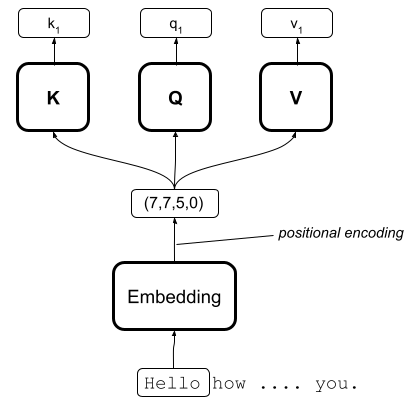
\includegraphics[scale=.4]{./images/transformerBlockBasic.png}
\caption[Jeff Yoshimi with consultation from Tim Meyer.]{Part of a transformer block. Each token in the context window is converted into a vector using the word embedding, then transformed using the positional encoding. This vector is then multiplied by three matrices $\textbf{K}$, $\textbf{Q}$, and $\textbf{V}$ to produce three vectors. These operations can be done concurrently and can thus run on fast parallel computing hardware. The resulting vectors will be used to produce a representation that captures relationships between items in the context window. Bolded items are matrices that are updated using gradient descent.}
\label{transformerBlockSimple}
\end{figure}
% More on normalizing. See neuralnets.txt. Also need a picture to show that input and output are same-sized.

The details of what occurs in a block are not developed in detail here though we are planning to expand the discussion in future versions of this chapter. However, here is a rough sketch of what happens. Each input token in a context window is first converted into a vector using a vector embedding (chapter \extref{ch_word_embeddings}). This vector is then simultaneously matrix multiplied by three weight matrices labeled $\textbf{K}$, $\textbf{Q}$, and $\textbf{V}$ to produce three vectors: the key, query, and value vectors. This is what is shown in figure \ref{transformerBlockSimple}. Note that the matrices, in bold, are part of what is trained in this architecture.

% More on normalization, "scaled dot product"
The key and query vectors are then multiplied (using a dot product) in all possible combinations and then normalized to produce a context representation. This is shown in figure \ref{selfAttention}. These are also called self attention scores. These scores capture relationships between tokens in a context window. The value vectors (not shown in figure \ref{selfAttention}) are then matrix multiplied by the self-attention matrix to produce the outputs of one attention head of a transformer layer.

\begin{figure}[h]
\centering
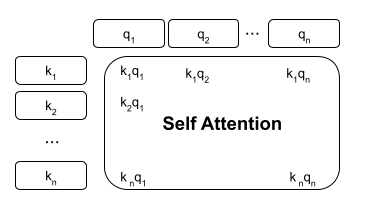
\includegraphics[scale=.6]{./images/selfAttention.png}
\caption[Jeff Yoshimi with consultation from Tim Meyer.]{Scaled self attention matrix generated by multiplying key and query vectors (using the dot product). Value vectors (not shown) are then multiplied by this matrix to produce the output of one head of a block.}
\label{selfAttention}
\end{figure}

% Eric S: At multiple heads: Can you explain a bit more in ordinary language what the functional importance of these transformation is?  Maybe some examples would help. What kinds of things generate high vs low self-attention?
Within each block all the mechanisms above are separated into multiple attention ``heads''.  That is, the $\textbf{K}$, $\textbf{Q}$, and $\textbf{V}$ matrices project from the embedding dimension to a head dimension.\footnote{This is roughly the number of embedding dimension divided by the number of heads so that when the outputs are concatenated we get back to the same dimension. This can be seen in figure \ref{gptParams}, where the number of inputs to each head, $d_\text{head}$, is equal  or almost equal to  the embedding dimension $d_\text{model}$ times the number of heads $n_\text{heads}$.}  For example if the embedding dimension were 9 it might get reduced to three 3-dimensional heads.\footnote{Thus for each head the $\textbf{K}$, $\textbf{Q}$, and $\textbf{V}$ matrices are shaped accordingly, here $9 \times 3$ with 9 rows for the inputs from the embedding (or a previous layer) and 3 columns for the outputs (into the heads). In practice rather than having separate $\textbf{K}$, $\textbf{Q}$, and $\textbf{V}$ matrices for each head they are combined into a single matrix for efficiency.}
% Mention slicing as a way of extracting a subset of elements from an array, matrix, or tensor.
% The query asks a kind of question, and the key is a kind of answer. See 3b1b. 

As a result of this multi-head attention, the network can learn \emph{multiple} ways to compare words in the sentence to each other, a bit like how a convolutional network (section \extref{convolutionalLayer}) develops \emph{multiple} filters to analyze an image. The results of these different attention heads are combined and as a result each layer of a transformer network involves a sophisticated representation of the sentence that represents multiple types of inter-word dependency. The number of heads per block corresponds to a more complex form of representational width.

% This part is not clear yet. Also, the figure should probably have ``de-embedding'' and ``softmax'' in the final layer separate from the FF part somehow.
This entire process happens once for each head. The outputs of all the heads are then concatenated back together and normalized, and put through a standard feed-forward network of the kind we've been talking about throughout the book.\footnote{Residual connections are also used. That is, the input to the block is added directly to the output of the multi-head attention mechanism. This allows the gradient descent algorithm to have a direct route backwards through the blocks of the network, as a way to address the vanishing gradient problem (see chapter \extref{ch_supervised_recurrent}). }  The output of the block is a set of vectors that has the same shape as the input vectors. See figure \ref{transformerArchitectureSchematic}. For example, in the example in figure \ref{contextWindow} the input would be 9 vectors with 4 components each, and the output would be too. For a nice visualization that is vaguely in the Simbrain style, see \url{https://bbycroft.net/llm}.
% Discuss how the input and output sizes stay the same through the layers. According to GPT this is for multiple reasons (simple design and stacking, facilitate residual connections, stable layer normalization, uniform attention mechanism).

\begin{figure}[h]
\centering
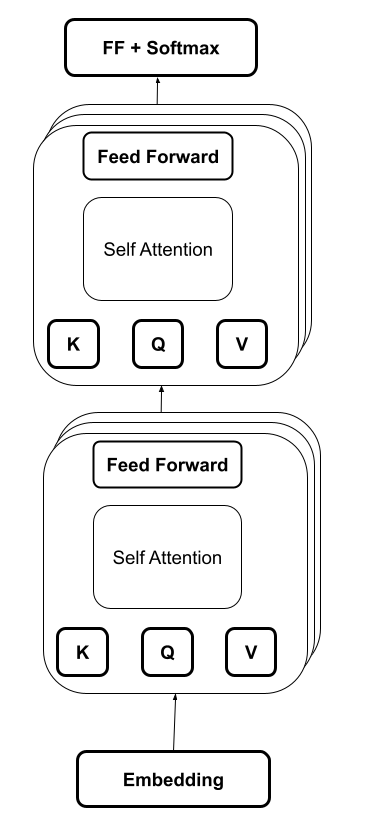
\includegraphics[scale=.35]{./images/transformerArchitectureSchematic.png}
\caption[Jeff Yoshimi with consultation from Tim Meyer.]{Schematic of the transformer architecture. Multiple blocks are stacked, capturing representational depth, as in a CNN. Each block contains a multi-head attention structure, where each head learns to represent inputs to the block in a different way. This captures representational width. The outputs of the multiple heads are combined in a standard feed-forward network. Other structures handling residual connections, and adding and norming activations, are not shown. As above bolded items contain trainable parameters that are updated via gradient descent.}
\label{transformerArchitectureSchematic}
\end{figure}
 
Now we take a lesson from deep networks, and stack many of these transformer blocks on top of each other, to produce increasingly sophisticated representations. This is representational depth. Recall that with deep networks for vision, we get features, features of features, features of these features, etc. whose activations match neural response properties of different layers of the human visual system. This builds on the old idea of the \emph{Pandemonium} model (section \extref{cog_rev}), which involved (at successive layers): edge detectors, detectors for combinations of edges, detectors for combinations of these combinations (e.g. fragments of letters), and ultimately letter detectors. In a similar way, the successive layers of a transformer model of language correspond to increasingly complex features of the input stream, including syntactic categories, semantic properties, and far more complex features as well.\footnote{The extent to which activation patterns correspond to syntactic or semantic features is measured using post-hoc interpretation techniques such as probing. As with so many other neural network features, these were not ``programmed in'' by the engineers, but are emergent from the network after training, and are studied and described by scientists after the fact.}

The whole thing is trained using gradient descent and supervised learning (chapter \extref{ch_supervised}). It's the same ideas as with a simple feed-forward network, but with more components trained. Items in bold in the figures above are trained: the word embedding, the key, query, and value matrices for each head in each block, and the normal weights and biases of the feed-forward networks. Gradient descent is being pushed back through a \emph{lot} of stuff here!

\subsection{Softmax Outputs}\label{llmOutput}

The first step in a transformer is to embed inputs, as we've seen. The last step is to un-embed them. 

In figure \ref{nextWordPrediction} to make it clear that we were predicting the next word in a sequence, we just showed the same word embedding in the input and output. However, it turns out that in practice, one-hot encodings over the whole vocabulary are used as targets (that is, patterns that consist of all zeros and a single ``hot'' one; see section \extref{wrangling}). When target data are binary one-hot encoded labels, the task given a network is technically a classification task (section \extref{classificationRegression}). Thus transformers are technically classifiers, which classify input texts according to what word is likely to occur next. Classification can here be seen as serving as a \emph{proxy task}. Our actual task is to predict a set of probabilities over next tokens. The output of an LLM is a set of probabilities over next tokens.\footnote{The interesting thing is that by \emph{trying} to perfectly classify next tokens (an impossible task), we end up with good probabilities, which is exactly we're after. Here is a way to think of it. If the model was trained to 100\% accuracy on the classification task, then it would always generate the same sentences from the same prompts (because it would assign one unique token to the current input). But then it could not generate new instances of text.}

The output of an LLM is often a \glossary{softmax} layer with around 50,000 outputs,  which  indicate how probable a token is given the input (all the prompts and responses in the context window so far ). See figure \ref{contextWindow} for how this might look for our simple example, where the output vocabulary just contains 7 tokens.

\begin{figure}[h]
\centering
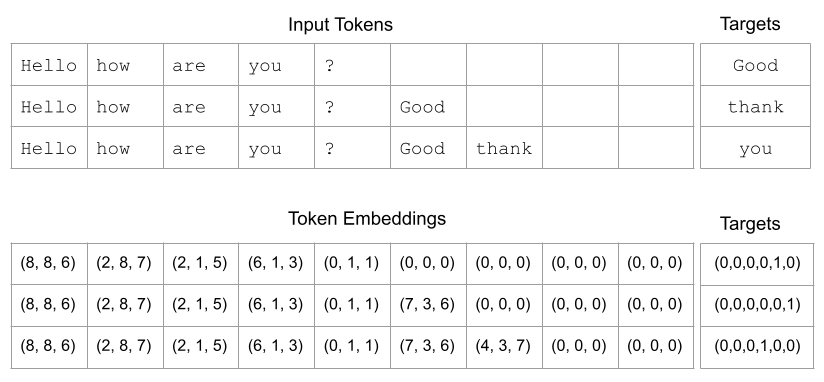
\includegraphics[scale=.45]{./images/contextWindow.png}
\caption[Jeff Yoshimi]{What some training data might look like for the example in figure \ref{gptRecursedInputs}. The top panel shows the tokens in three training examples and the bottom row shows the corresponding token embeddings. The bottom panel shows inputs that can actually be fed into a neural network, in this case, a network with $9 \dot 4 = 36$ input nodes. Note that the targets are one-hot encoded, because these networks are actually classifiers (see section \ref{llmOutput}). Thus the output layer in this simple network would have 7 nodes for the 7 tokens: ``Hello'', ``how'', ``are'', ''you'', ``?'', "Good'', ``thank''. The softmax outputs are not shown, but for a well-trained network the outputs would be probability distributions close to the targets, for example $(0,0,.01,0,.99,0),  (.01,.01,0,0,0,.98), (0,.01,0,.98,0,.01)$. On softmax see section \extref{wta_softmax_section}}
\label{contextWindow}
\end{figure}

% Tim says it would be really nice to have this as a system diagram or like the multi head diagram above.
Once we have a probability distribution over tokens, we select one of the most probable next tokens and that becomes the output. This is usually done by sampling from among the top $n$ most probable next tokens. This can be controlled using the softmax temperature parameter, where higher temperatures make the outputs more random or ``creative'' (see section \extref{wta_softmax_section}). Thus the final softmax layer does the opposite of what the embedding layer does. Rather than converting from tokens to activations, it converts from activations to tokens, and is thus a ``de-embedding'' layer.

\subsection{Parameters and hyperparameters}

By way of summarizing, consider the parameters and  \glossary{hyperparameters} associated with a transformer-based LLM. Recall that parameters are primarily weights and biases. Figure \ref{gptParams} shows this for a range of GPT-3 subvarieties as $n_\text{params}$. The released version of GPT-3 had 175 Billion weights and biases. By comparison, our xor 2-2-1 network had 3 biases and 6 weights, or 9 parameters. A standard convolutional neural network might have millions of parameters. So this is just massively larger. Of course things have gotten larger. GPT-4 has about 1.76 trillion parameters. It takes large server banks that  consume huge amounts of energy to run these models, and so there is a thread attempting to achieve similar performance with smaller models, some of which can be run on a  person computer.\footnote{For example, Gemma2B achieves performance similar to GPT 3.5 with 2 billion parameter. See \url{https://developers.googleblog.com/en/smaller-safer-more-transparent-advancing-responsible-ai-with-gemma/}.}

Hyperparameters are values that describe the structure of a model. For a simple feed-forward network the main hyperparamters correspond to the number of layers and nodes per layer. For a transformer, they correspond to the number of layers $n_\text{layers}$, dimension of the word embedding $d_\text{model}$, number of attention heads $n_\text{heads}$\footnote{Notice that the size of the heads, $d_\text{head}$ is equal or almost equal to  $d_\text{model} \times n_\text{heads}$ (some mismatches are allowed).}, a batch size, and a learning rate. Even if the details of how transformers work is difficult, you should know enough to interpret this table. Certainly learning rate and batch size are values we've seen in other chapters.

\begin{figure}[h]
\centering
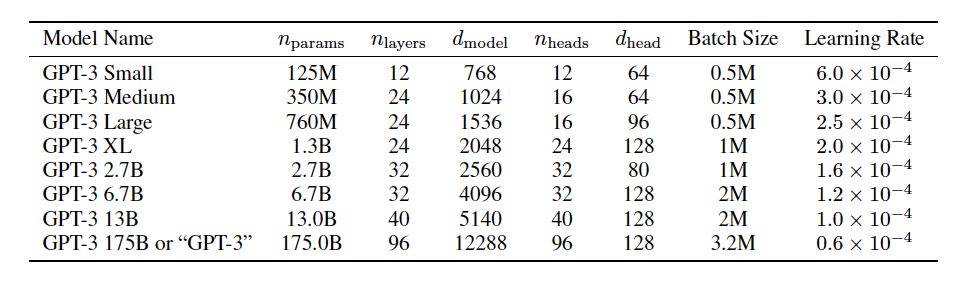
\includegraphics[scale=.4]{./images/gpt3_params.png}
\caption[\url{https://arxiv.org/abs/2005.14165}.]{Number of parameters and values for some of the hyperparameters used in training different versions of GPT-3. }
\label{gptParams}
\end{figure}

The size of the context window is another hyperparameter not shown in the figure. According to ibm research, ``when ChatGPT made its debut nearly two years ago, its window maxed out at 4,000 tokens. If your conversation went over the 3,000-word chat-interface limit, the chatbot was likely to hallucinate and veer off-topic. Today, the standard is 32,000 tokens, with the industry shifting to 128,000 tokens, which is about the length of a 250-page book. IBM just open-sourced on Hugging Face two Granite models with a 128,000-token window, and more are on their way.''\footnote{\url{https://research.ibm.com/blog/larger-context-window}.}

% TODO: New section. Something like "Other features of LLMs"

%One shot, zero shot etc. Lots of the "shot" learning is based on reasoning  (through the width and depth of the giant network), getting it to reason step by step through something. It is not weights and biases. Background of one shot in AI vs. NN. NN require gradual learning but humans learn in one shot so that was a problem. And classical AI can do so too just with a single rule in the databas

% Prompt engineering, pre-training, adaptation tuning, utilization, and capacity evaluation.
%
% Fine tuning. Fine tuning is updating an already existing LLM to bias it in favor of the language in some specified corpus you are interested in. For example you might download a llama 2 model, and then fine tune it based on a set of corpus using x library. See Kauf and Ivanova 2023
% Video on fine tuning an LLM to talk about a set of PDFS (we can do it on Husserl): https://www.youtube.com/watch?v=dXxQ0LR-3Hg
%
% In context learning are things you can add to your prompt, ie in the context window, to improve the output, will be discussed further in the prompt engineering chapter
% 
% Use of external functionalities like wolfram alpha
%
% Prompt engineering. Prompt templates. Prompting techniques. Funny historical examples of prompting discoveries
%
%https://developer.nvidia.com/blog/how-to-get-better-outputs-from-your-large-language-model/
%
%https://arxiv.org/pdf/2310.14735.pdf
%

\section{Analysis of LLMs}\label{llm_analsis}

As with all the architectures discussed in this book, transformer-based LLMs are not just used to engineer useful devices but are also major object of scientific interest (see chapter \extref{ch_applications}). They are studied in many academic disciplines and areas of cognitive science. They are in various ways being considered as models of cognition, linguistic processing, and neural processing. 

% A difference in degree not kind. (A few points are mixed together here). It was not clear they would generalize so well. So a link to that. Can ask about situations etc. (See the dreyfus point). Pierre thought the best that would happen is grammar. (Jeff immediately tried old Dreyfus experiments and it passed). 
These models have the remarkable property of being human engineered but not completely understood by the humans who engineered them (this is true of other models, but is especially the case here, given how complex LLMs are, and given how expensive they are to train). 
% Add some condensation of "LLMs being human-built but still of interest to science" below.

Here are some representative examples of recent research into LLMs. Here again, the landscape is rapidly changing, and this section will have to be frequently updated.

\subsection{LLMs and Cognitive Science}\label{llm_cogsci}

A theme running through this book is that cognitive scientists are interested in neural networks, even when they originate in fields outside of cognitive science. That trend has continued with the emergence of large language models.

Cognitive scientists studying language took an interest in BERT, an early LLM that came out around the time of GPT ``1'' (2018). A problem for earlier accounts of language processing was that they could not handle long-range dependencies in texts. In a paper co-authored by Jay McClelland  \cite{mcclelland2020placing} (a member of the original PDP group at UCSD; see section \extref{first_resurgence}), the following example is used to illustrate the point:
\begin{quote}
John put some beer in a cooler and went out with his friends to play volleyball. Soon after he left, someone \textbf{took the beer} out of the cooler. John and his friends were thirsty after the game, and went back to his place for some beers. When John opened the cooler, he discovered that the beer was \rule{1cm}{0.15mm}.
\end{quote}
What the reader expects in the blank spot  depends on text earlier in he sentence. Here the reader expects the word ``gone'' next, but if ``took the beer'' is replaced with ``took the ice'' the reader expects something like ``warm''. McClelland and colleagues also considered how these models shed light on cognitive modelings and brain regions. Others have taken this kind of study much further since then.

Among current interests are papers that show that LLM representations are aligned with neural activations,  perceptual spaces,  physical spaces and conceptual spaces. Caucheteux et al. show that language model activations predict up to 40\% of brain activity during language processing \cite{caucheteux2022brains}. Abdou et al. demonstrate that language models can encode perceptual color relationships, even though they have never ``seen'' colors the way sighted humans have (but have only read about color relationship in texts) \cite{abdou2021can}. Liétard et al. find that LLMs can predict relative geographic distances between cities \cite{lietard2021do}. Christiansen et al. report that LLMs organize concepts in ways that correlate with human conceptual structures \cite{christiansen2023large}. These findings collectively suggest that LLM representations are not ``empty symbols'' as in traditional computer programs (see the discussion in \extref{classicalAIComparison}). Instead, they are content-rich and structured similarly to human mental representations.

Given these results, it seems likely that a lot of future research on LLMs will contribute to the field of cognitive science. Conversely, the acquired findings of cognitive science also contribute to research on LLMs. Notably, these findings are used to better measure the cognitive abilities of LLMs. One of the tasks of the main LLM benchmark BIG-BENCH, notably draws on cognitive science to test the ability to understand and combine concepts, including novel and made-up ones \cite{srivastava2022beyond}.

\subsection{LLMs and Linguistics}

Linguists have considered how these models handle syntax and semantics, revealing insights that bridge computational models and linguistic theory. One key study (``What Does BERT Look At? An Analysis of BERT's Attention'') investigates the attention patterns in BERT and their correspondence to linguistic phenomena. This study found that BERT's attention heads often focus on specific linguistic roles, such as the direct objects of verbs or the determiners of nouns. Interestingly, some attention heads display broad attention across entire sentences, while others are highly focused, suggesting a complex, multi-faceted approach to language understanding within the model. 

\subsection{LLMs and Neuroscience}

Just like Yamins and DiCarlo used convolutional neural networks (CNNs) to predict brain activity (section \extref{cnn_applications}), researchers are now leveraging transformer-LLMs to understand how our brains process language. 

Schrimpf and colleagues \cite{schrimpf2021neural} explore how LLMs, like GPT and BERT, can predict neural responses during language comprehension. They proceeded by comparing  brain activity of participants reading or listening to sentences with the activity patterns generated by these models. One of their key findings is that transformer models, especially GPT, can predict nearly 100\% of the explainable variance in neural responses to sentences! 

% Work and cohere with any material added on BERT
An interesting aspect of this study is the comparison between GPT and BERT. GPT, which processes language in a unidirectional manner (predicting the next word based on the previous words), was found to outperform BERT, which uses a bidirectional approach (considering the context from both directions). This suggests that our brain predicts unidirectionally, which  makes sense given that we usually are confronted with language orally and so get ``fed'' sentences word by word. 

% Removed given Eric S comments
%This provides some evidence for a theory of neuroscience called \emph{predictive processing}, which suggests that the brain is constantly making predictions about incoming sensory information to enable us to navigate the world.

\subsection{LLMs and Philosophy}\label{llmPhilosophy}

% Cite Chomsky's reaction to all this
Philosophers are also interested in LLMs for the obvious reason that they have completely changed the game and even passed the Turing Test. But do they understanding language?\footnote{This is a throwback to the old AI-connectionism debate (section \extref{cog_rev}), and one way to think about the current debate is as a revival of that one.} One line of argument is that a machine can’t get the ``meaning'' of a word just by manipulating meaningless symbols. After an article by Emily Bender and colleagues \cite{bender2021dangers}, it has become common to say that LLMs are mere ``stochastic parrots'' that capture nothing more than mere co-occurrence probabilities. 

These arguments have a long pre-history in what are sometimes called \emph{unusual realization arguments}. These arguments
\begin{quote}
ask us to imagine people carrying out simple operations on bit streams, connectionist-like computations on activations patterns, or the control operations of the central processing unit of a computer. For example, Dneprov asks us to imagine a stadium full of people who pass 0’s and 1’s to one another on the basis of instructions announced over a loudspeaker. We can further imagine that this stadium is linked to an input-output device that enables it to pass the Turing test. We can then ask ourselves: do we really think this stadium full of people has consciousness or genuine understanding? \cite{noelle2022artificial}
\end{quote}

Bender and Koller have adapted these arguments to LLMs using an ``Octopus test'' \cite{bender2020climbing}, which goes like this: two English-speaking castaways communicate via telegraph across islands. A super-intelligent octopus intercepts their messages, learns the statistical patterns of the messages going back and forth, and, ``feeling lonely'', inserts itself into the conversation. The question is whether they would be able to convince the interlocutors they were intelligent-- a version of the Turing Test. Bender and Koller argue that the octopus could pass the test for simple chatbot like interactions, but that it would fail in responding to strange situations involving words referring to objects the octopus has never perceived. This scenario is used to argue that, like the octopus, LLMs may produce seemingly meaningful outputs based solely on statistical patterns, without true understanding of language or the concepts they appear to discuss.

\begin{figure}[h]
\centering
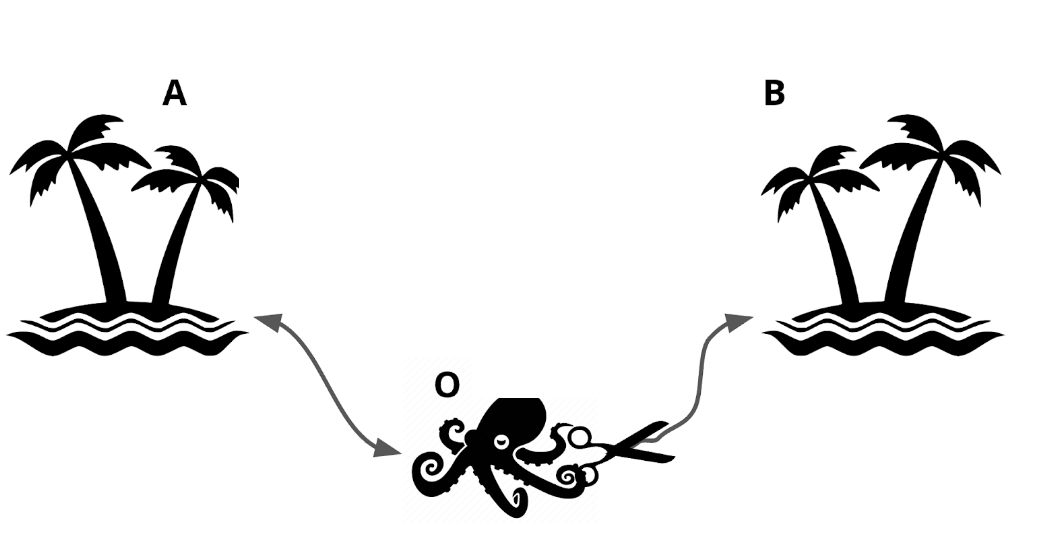
\includegraphics[scale=.20]{./images/octopusTest.png}
\caption[Soraya Boza.]{The octopus test. In the upper panel the octopus is observing the information being passed back and forth. At a certain point the octopus intercepts the wire and starts passing statistically similar messages to the person on the first island. This is shown in the lower panel. The communication is convincing, and the person on the left does not realize what has happened (the poor person on the right is just out of luck at this point). It has been argued that the octopus would not understand the information it passed along, even if it was convincing to the human. Moreover, it has been argued that the octopus would fail to produce convincing text in certain novel situations.}
\label{octopusTest}
\end{figure}

However, others argue that LLMs do understanding the meaning of words they produce. Relying on findings presented in section \ref{llm_cogsci}, Sogaard \cite{sogaard2023grounding} argues that the representations LLMs rely on are grounded (that is, they are meaningful) in virtue of their alignment with human cognitive and perceptual spaces. These are not like the empty symbols passed along in Dneprov's stadium or in other ``unusual realization arguments.'' Here, the LLM (or the octopus) manipulates representations that have internal structures aligned with those of the human mind. In any case, the impressive results of models such as chatGPT fundamentally question not only empirical insights about language but also very deep philosophical conceptions about language.

Another long-standing argument against machine intelligence due to Hubert Dreyfus \cite{dreyfus1992computers} is that no computer or neural network could ever have truly human capacities, because they were not raised in the real world and can only parrot back what they were programmed or trained to say, at best with moderate abilities to generalize beyond that (Bender and Keller's argument develop this idea with respect to LLMs and argue these considerations are why the octopus would pass the test). However, humans with their embodied human existence develop an intuitive sense of the full context of the lived world. To show this, one of the authors (Yoshimi), who has regularly taught Dreyfus'  argument for many years, would have the class ask strange or unusual questions to AI systems and chatbots of earlier years, like "What would happen if a penguin were to juggle alligators." The systems invariably struggled to say anything meaningful (though some did well by tricks, like pretending to be a teenager saying ``lol who cares''). But chatGPT does just fine with the question, as you are welcome to see for yourself. Not everyone is convinced by this, and the discussion remains active. Melanie Mitchell \cite{mitchell2021ai} has argued that despite appearances, these systems are not as intelligent as they appear (there are many reasoning tasks they fail on, for example).

% Discussion of LLMs being human-built but still of interest to science.

%There is something strange about LLMs. They were built by humans but are so complex that we do not completely understand them. This has often been the case historically with neural networks, but the issue is accentuated here. It's like we built this super powerful motor and now we can put it in different things, but we don't understand how the motor works so we have to look at its components and find new ways to study it, reverse engineer it, use it, etc. This may be a difference of degree (CNNs were also like this), but it is enough of a difference in degree that it feels like a change in kind.\footnote{One aspect of this is that with CNN's one could run a bunch on their own computer; with LLMs they are so expensive to train and it takes so long that people just make API calls to existing LLM models. So it feels more like this separately existing thing is just being studied, akin to studying any natural phenomenon in nature.} It really does feel different. These massive transformer-based neural networks with all their many layers and blocks and matrices and other features somehow magically produce human-like speech and video, etc., but how exactly is not understood. 
% 
%This is a twist on our earlier discussion of types of neural network research (chapter \extref{ch_applications}). It was built for engineering, but ended up being useful for science. Most earlier cases started in science and went to engineering (e.g. deep learning CNNs).
%
%The point was made striking early via BERT (which came out around the time of GPT-2). It came out of Google and fit their engineering needs. Psychologists and linguists then realized  BERT was doing better at analyzing language than other models in linguistics, so they started to treat it as an object of scientific interest in its own right. This gave rise to a new field called ``BERTology''. 
%
%As a result of this feature of LLMs, a huge ecosystem of analysis is growing up around them. Not all of it is obviously relevant to our focus here, cognitive science, but much of it is potentially relevant and it's too early to tell, so we here give a brief review.

%Engineers built something and then scientists created a science to understand it! In \cite{rogers2020primer} the authors explain:
%\begin{quote}
%Although it is clear that BERT works remarkably well, it is less clear why, which limits further hypothesis-driven improvement of the architecture. Unlike CNNs, the Transformers have little cognitive motivation, and the size of these models limits our ability to experiment with pre-training and perform ablation studies. This explains a large number of studies over the past year that attempted to understand the reasons behind BERT’s performance. In this paper, we provide an overview of what has been learned to date, highlighting the questions that are still unresolved.
%\end{quote}


